\documentclass[11pt]{article}

\newif\ifpdf
\ifx\pdfoutput\undefined
\pdffalse % we are not running PDFLaTeX
\else
\pdfoutput=1 % we are running PDFLaTeX
\pdftrue
\fi

\ifpdf
\usepackage[pdftex]{graphicx}
\else
\usepackage{graphicx}
\fi

\usepackage{setspace}
\doublespacing

\textwidth = 6.5 in
\textheight = 9 in
\oddsidemargin = 0.0 in
\evensidemargin = 0.0 in
\topmargin = 0.0 in
\headheight = 0.0 in
\headsep = 0.0 in
\parskip = 0.2in
\parindent = 0.0in


\newtheorem{theorem}{Theorem}
\newtheorem{corollary}[theorem]{Corollary}
\newtheorem{definition}{Definition}

\title{PyTrilinos: Recent Advances in the \\ Python Interface to Trilinos}
\author{William F. Spotz \\ Sandia National Laboratories, Albuquerque, NM}
\begin{document}

\ifpdf
\DeclareGraphicsExtensions{.png, .pdf, .jpg, .tif}
\else
\DeclareGraphicsExtensions{.eps, .jpg}
\fi

\maketitle

\begin{abstract}
PyTrilinos is a set of Python interfaces to compiled Trilinos packages.  This collection supports serial and parallel dense linear algebra, serial and parallel sparse linear algebra, direct and iterative linear solution techniques, algebraic and multilevel preconditioners, nonlinear solvers and continuation algorithms, eigensolvers and partitioning algorithms.  Also included are a variety of related utility functions and classes, including distributed I/O, coloring algorithms and matrix generation.  PyTrilinos vector objects are compatible with the popular NumPy Python package.  As a Python front end to compiled libraries, PyTrilinos takes advantage of the flexibility and ease of use of Python, and the efficiency of the underlying C++, C and Fortran numerical kernels.  This paper covers recent, previously unpublished advances in the PyTrilinos package.
\end{abstract}

{\bf Keywords:} Trilinos, Python, sparse linear algebra, parallel programming, nonlinear solvers, eigensolvers, partitioning, preconditioners.

\section{Introduction}
\label{sec:introduction}

Python is an increasingly popular language for scientific computing.  NumPy~\cite{NumPyGuide} (Numerical Python) provides an extremely convenient, high-level interface to homogeneous, contiguous (and non-contiguous) arrays of data.  SciPy~\cite{SciPyRefGuide} (Scientific Python) is built on top of NumPy and provides a Python interface to many of the most popular scientific libraries available.  Matplotlib~\cite{Matplotlib} provides high-quality plotting capabilities.  Parallelism is available via a long list of open source modules.  Robust solvers are provided by the Python interfaces to PETSc~\cite{PETScUserRef} and Trilinos~\cite{Trilinos}.  The SciPy Conference~\cite{SciPyConference} continues to grow in popularity, and the presence of several Python sessions at scientific computing conferences such as SuperComputing~\cite{SuperComputing} and the SIAM Conference on Computational Science and Engineering~\cite{SIAM_CSE} attest to the strong interest in using Python for scientific programming.  In fact, Python is now seen as a credible open source competitor to MATLAB~\cite{MATLAB}, perhaps the single most popular platform for small to medium scale scientific computing.  This is in part because Python and MATLAB share certain traits in common: they are both high-level, interpreted, interactive and dynamic.

At the other end of the scientific computing spectrum are compiled codes written in Fortran, C and C++ that run on massively parallel architectures to solve large, multiscale, multiphysics problems.  These codes utilize low-level languages in an attempt to achieve near-optimal processing efficiencies.  While the success at achieving this goal is debatable, there is no question that compiled languages are more efficient than interpreted languages such as Python.

As the complexity of simulations increases, however, more and more code is devoted to setup and to initialization of a series of subproblems that must all interface together to describe the larger scientific problem.  This ``command and control'' software can dominate the numerical kernels in terms of total lines of code, while the kernels themselves still dominate runtime execution.  Low-level languages are notoriously ill-suited to these types of bookkeeping tasks.  It is therefore easy to make the case that low-level languages should handle the numerically intense kernels and high-level languages should be utilized for command and control.

This perhaps explains the rise in popularity of Python for scientific computing.  As a high level, object-oriented language, it is very well suited to the high-level description of scientific problems, to provide the modularity so often sought by scientists asking ``what if'' questions, and to glue together the various components (often developed in different low-level languages) of a successful scientific simulation.  A well designed scientific Python code will hand off the numerically intense computations to optimized compiled code, while maintaining usability, readability and developmental scalability at the highest level.

PyTrilinos provides just such a capability.  It supports massively parallel vector and multivector objects and massively parallel operators such as sparse matrices.  PyTrilinos also supports solver algorithms that utilize these objects, enabling the development of complex codes with convenient Python interfaces and efficient Trilinos algorithms.  For example, FiPy~\cite{FiPy,FiPy_Site} and FEniCS~\cite{FEniCS} are both Python-based partial differential equation solvers that provide PyTrilinos solvers as an option and HYPO4D~\cite{HYPO4D} is currently being refactored to use Python and PyTrilinos.  This paper details recent advances in the PyTrilinos package, including its new documentation system, recently added Trilinos modules, a focus on improvements to the Teuchos module, and model evaluators.  We finish with a vision for interfaces to second-generation Trilinos packages.

\section{Review}
\label{sec:review}

The first PyTrilinos article~\cite{PyTrilinos}, published in 2008, described the status of the project circa 2007.  In order to put recent advances in context, we begin with two reviews: first, a review of the historical origin of PyTrilinos, and second, a review of the topics covered and conclusions drawn in the first PyTrilinos article.

\subsection{The Origin of PyTrilinos}
\label{sec:origin}

The author --- lead developer of PyTrilinos --- was introduced to Python for scientific computing by a colleague.  The project was to develop a framework for testing new ideas for fully implicit multiphysics coupling using Jacobian Free Newton Krylov (JFNK)~\cite{JFNK}.  The JFNK idea starts with Newton's algorithm to find $\mathbf x$ such that nonlinear function $\mathbf F(\mathbf x) = 0$, where successive iterates are computed by
\begin{eqnarray}
  \label{eqn:innerSolve}
  \mathbf F(\mathbf x^n) & = & -\mathbf F'(\mathbf x^n) \Delta\mathbf x^n , \\
  \mathbf x^{n+1} & = & \mathbf x^n + \Delta\mathbf x^n,
\end{eqnarray}
where $\mathbf F'$ is the Jacobian of $\mathbf F$.  Equation~(\ref{eqn:innerSolve}) is a linear system that must be solved for $\Delta\mathbf x^n$ and JFNK utilizes Krylov space methods to iterate to a solution.  Krylov methods share the characteristic that we need only be able to compute  the matrix vector product for arbitrary vector $\mathbf v$, in this case $\mathbf F'(\mathbf x) \mathbf v$.  This quantity, known as the directional derivative, can be approximated without computing and storing the Jacobian via
\begin{equation}
  \label{eqn:directionalDerivative}
  \mathbf F'(\mathbf x) \mathbf v \approx \frac{\mathbf F(\mathbf x + \delta\mathbf v) - \mathbf F(\mathbf x)}{\delta}
\end{equation}
for appropriate values of $\delta$.  For a coupled problem, we can set $\mathbf F = (\mathbf F_1^\mathrm{T}, \mathbf F_2^\mathrm{T}, \ldots)^\mathrm{T}$ and $\mathbf x = (\mathbf x_1^\mathrm{T}, \mathbf x_2^\mathrm{T}, \ldots)^\mathrm{T}$, and Equations~(\ref{eqn:innerSolve}--\ref{eqn:directionalDerivative}) then represent a coupled solver.

The coupled solver idea was inherently object-oriented: there would be a collection of (simple at first) physics modules (to compute $\mathbf F_1$, $\mathbf F_2$, $\ldots$) that could be plugged into a higher-level solver object capable of building a fully coupled system, depicted in Figure~\ref{fig:CoupledSolver}, that could be solved by JFNK.  It would require abstract concepts such a "unknowns" made concrete and a bookkeeping system to keep track of them, and by extension, keep track of how the different physics modules were coupled to each other.

\begin{figure}
  \begin{center}
    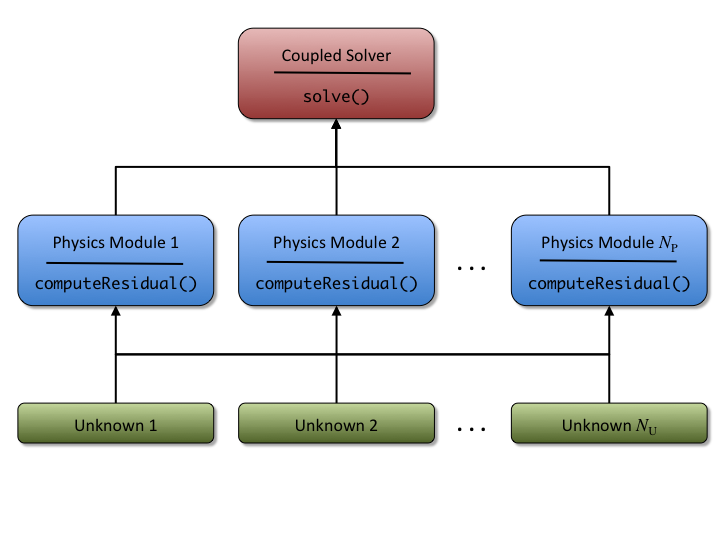
\includegraphics[width=5.5in]{CoupledSolver}
    \caption{Conceptual design of the coupled solver.  The unknowns typically represent different fields.  The physics modules represent equations.  Not all equations utilize all unknowns.  The coupled solver {\tt solve()} method requires each physics module to compute its residual via its {\tt computeResidual()} method.}
    \label{fig:CoupledSolver}
  \end{center}
\end{figure}

This research was being conducted at a time when Sandia was one of the few American laboratories that had ventured into object-oriented programming for scientific computing.  One of the early lessons learned was that object oriented design was non-trivial.  It was easy to make things more complicated than necessary, and it was easy to miss design elements that could eventually become crucial.  It was common to refactor a design once, twice, or three times before settling on a design that supported the necessary set of features.  Often (but not always) a refactor would require completely throwing away the previous iteration.  In this environment, the following statement was hard to argue with: ``If you are going to throw away early iterations, why not write them in Python, which is quicker and easier to write than C++?''

So it was under this philosophy that the decision was made to write the first version of our multiphysics coupler in Python.  The result was somewhat revelatory: we developed a simple mesh class, field classes that represented both knowns and unknowns, a physics module base class and two concrete physics module derived classes, a multiphysics coupler base class and an explicit derived solver, all in one day using Python.  The physics modules represented the two Brusselator equations,
\begin{eqnarray}
  \frac{\partial X}{\partial t} & = & D_1 \nabla^2 X + a - (b+1) X + X^2 Y, \\
  \frac{\partial Y}{\partial t} & = & D_2 \nabla^2 Y + b X - X^2 Y,
\end{eqnarray}

which in this initial case were 1D diffusion equations with nonlinear forcing functions.  The explicit solver implemented simple, explicit forward Euler time stepping, which was a first step towards the implicit solvers that we were ultimately interested in.  After an additional half day of debugging, we were getting results.  Python had proven itself as a development tool beyond our expectations.

The next step was to derive a solver class that implemented implicit solves such as backward Euler or Crank-Nicolson.  This required a nonlinear solver implemented or wrapped in python that was robust enough to handle a large number of unknowns.  There were none available at that time.  We knew we wanted to test these multiphysics coupling ideas with Trilinos, so that the resulting capabilities could be folded into the larger project.  So we had a choice: wrap the needed components of Trilinos to be accessible from Python, or rewrite the coupling framework in C++.  Our initial experience with Python had been so favorable that PyTrilinos was born.  This required a Python interface to NOX, the nonlinear solver package.  NOX utilizes the concept of an abstract interface, but the primary concrete interface was for Epetra, and so Epetra also required a Python interface.  NOX uses other Trilinos packages: AztecOO for Krylov space iterative linear solvers, IFPACK for preconditioning, etc.  However, Python interfaces for these packages were not initially necessary.

Ultimately, the purpose of this framework was to test various preconditioning and scaling strategies within the context of a JFNK solver applied to coupled multiphysics.  The lessons learned from those tests were implemented in various Trilinos packages as well as full scale applications.  The Python framework was sufficient for running these tests and so a top-level C++ version was never written.  Conclusions drawn from the experience include:

\begin{itemize}

\item The time for development of scientific code can be significantly shortened using Python.

\item If you know you are in an iterative phase of code development, it is reasonable to view a future refactor as an opportunity to change to a compiled language, if that is what is warranted.

\item Scientific codes typically require sophisticated inputs.  Often, facilities for supporting this input begin to look like limited scripting languages.  A better approach is to start with a full-featured scripting language such as Python.

\item For our design, the numerical kernels ended up being {\tt computeResidual()} methods in Python classes derived from the {\tt PhysicsModule} base class.  The C++ NOX solver would actually call back to these Python methods during the solve.  See section~\ref{sec:capabilities} for a discussion of how to improve performance for this use case.

\item While our requirement was for a nonlinear solver, the utility of Python interfaces was apparent for other Trilinos packages such as linear solvers, preconditioners, eigensolvers, etc.

\end{itemize}

\subsection{Review of PyTrilinos Capabilities}
\label{sec:capabilities}

Here we review the capabilities covered in reference~\cite{PyTrilinos}.  The ``wrapper code'' necessary to provide the PyTrilinos interface is generated almost entirely by SWIG~\cite{SWIG_CXX_Python}, the Simple Wrapper and Interface Generator.  Other tools could have been chosen to facilitate this wrapping, including SIDL/Babel~\cite{Babel}, Boost.Python~\cite{BoostPython}, and more recently, Cython~\cite{Cython}.  All three of these tools require a manually written interface definition, which can fall out of sync with the wrapper source if the source interface changes.  This is perhaps the primary advantage of using SWIG to wrap Trilinos, which is a very large code base that is under active development.  The default SWIG behavior is to produce Python interfaces with a near one-to-one mapping to its C or C++ source code.  It was decided early in the PyTrilinos project that this was an appropriate approach for a code base as large as Trilinos.

The decision to use SWIG has largely been justified by the resulting development experience, with two exceptions.  The first exception is the handling of templated C++ code.  This was not an issue with first generation Trilinos code, but current Trilinos development is almost entirely templated, and so it must be addressed.  Section~\ref{sec:vision} covers this issue in more detail.  The second exception is nested classes, which is the one C++ construct that SWIG does not support.  Nested classes are utilized in the ModelEvaluator classes of the (wrapped) EpetraExt package and the (not-yet-wrapped) Thyra package.  This feature of SWIG required a significant workaround that undercut many of the advantages of SWIG.  Additionally, a common design pattern is iterators for containers, which are also typically implemented as nested classes.  In this case, the answer is to modify the Python interface to utilize Python iterators.  This is usually straightforward and results in a cleaner Python interface.

Because of its strong compatibility with NumPy (Numerical Python), PyTrilinos plays a role in a suite of mathematical and scientific Python tools that can be interpreted as an open source competitor to MATLAB.  This suite has the advantage of being free, of leveraging a more powerful scripting language, and of expanded interoperability with other languages.  PyTrilinos adds to this suite of tools implicit solver capabilities designed from the ground up for massively parallel computing.

At the time of publication of~\cite{PyTrilinos}, PyTrilinos provided interfaces to linear algebra services packages Epetra and EpetraExt; tools and testing packages Teuchos, Triutils, Galeri and New\_Package; direct and iterative linear solver packages Amesos and AztecOO; preconditioning packages IFPACK and ML; nonlinear solver package NOX; and continuation algorithms package LOCA.  Since this publication, PyTrilinos has released wrappers to eigensolver package Anasazi and complex linear algebra services package Komplex.  The most recent releases of Trilinos -- version 10.10 was released in February 2012 --- includes a new PyTrilinos package Isorropia, which provides parallel partitioning algorithms.  Support for New\_Package has been discontinued, as the purpose of this package is to provide a template for adding new packages to Trilinos, and its utility for new PyTrilinos packages was limited.

The PyTrilinos approach to enabling parallelism is to support the development of scripts that can be run in parallel in the standard way for a given parallel architecture.  For example, a parallel script can be run in an MPI environment on four processors using

\begin{verbatim}
    $ mpiexec -np 4 python myscript.py
\end{verbatim}

The {\tt myscript.py} script will in turn {\tt import} either the Teuchos or Epetra module (or both).  Both of these modules ensure that {\tt MPI\_Init()} has been called (with the latest releases of Trilinos, care has been taken to ensure that this behavior is compatible with other MPI Python interfaces such as pyMPI, PyPar or mpi4py).  Teuchos and Epetra provide abstract communicator classes as well as concrete implementations of these classes in the form of serial communicators and Message Passing Interface (MPI) communicators (and potentially others in the future).  These communicators are then used as the foundation for building other Trilinos objects, providing parallelism-awareness to all Trilinos objects that need it.  The Teuchos and Epetra modules also know to register the {\tt MPI\_Finalize()} command with the Python {\tt atexit} module when Teuchos or Epetra was responsible for calling {\tt MPI\_Init()}, thus ensuring a proper clean up.  On the other hand, if {\tt MPI\_Init()} was called before Teuchos or Epetra was imported, e.g. by mpi4py, then PyTrilinos assumes that the user is responsible for finalization.

Reference~\cite{PyTrilinos} contains comparisons between PyTrilinos and MATLAB for basic operations that are common to both.  The high-level conclusions are that MATLAB is more efficient at performing dense matrix vector multiplies and that PyTrilinos --- and Trilinos --- are more efficient at both sparse matrix vector multiplies and sparse matrix assignment.  These results reflect the different primary design objectives of the various tools.  It should be noted that this performance conclusion is drawn for comparisons that were made for operations in which the python interface introduced insignificant overhead compared to the C++ Trilinos interface.

Accordingly, PyTrilinos was also compared to Trilinos itself.  The primary usage differences are several: Python's dynamic object model versus the static typing of C++; memory management concerns present in C++ but not in Python; no header files in Python; and high-level containers in Python versus low-level C arrays.  The performance differences depend ultimately upon the granularity of the algorithm being tested.  Fine grained algorithms that do a lot of work (especially loops) in Python suffer significant performance penalties.  Coarse grained algorithms that hand off the bulk of the work to compiled routines can exhibit imperceptible performance hits in both serial and parallel.  Strategies for utilizing compiled code within a Python script include:

\begin{itemize}

\item Use high-level classes with pre-compiled kernels.  For example, the {\tt Epetra.CrsMatrix} class has a pre-compiled {\tt Multiply} method for performing sparse matrix-vector multiplication.  {\em Filling} the matrix values is a one-time initialization that would be performed in Python with a loop, but the multiplications (e.g., performed repeatedly within a solver algorithm) would be compiled.  This is in contrast to deriving from the lower-level {\tt Epetra.RowMatrix} base class and supplying a {\tt Multiply} method in Python.

\item Use NumPy array slice syntax to perform operations on ranges of data without an explicit Python loop.  For example, to compute the finite difference approximation to $\sigma = \partial u/\partial x$ on a uniform grid of mesh size $h$, we can fill all interior values of {\tt sigma} with

\begin{verbatim}
    sigma[1:-1] = (u[2:] - u[:-2]) / (2*h)
\end{verbatim}

which is much more efficient than looping over the elements of {\tt sigma} and {\tt u} in Python.

\item Use weave to compile embedded C/C++ code in Python.  For cases where loops in Python cannot be avoided, one option is convert the computational kernel to a Python string of C/C++ code and use the SciPy module weave to compile and use the code fragment.  In these cases, the prototype should be written in Python, and only after determining  that it constitutes a performance bottleneck, should weave be employed.

\item Write a Python extension module to handle computationally intensive algorithms.  Options include coding to the Python C API, or using the previously mentioned wrapper tools SWIG, SIDL/Babel, Boost.Python, f2py or Cython to automatically generate compiled Python extensions based on C, C++ or Fortran code. 
\end{itemize}

The advantages of PyTrilinos include rapid prototyping and brevity, due to the clean nature of Python syntax; and modularity and reusability, due to the scalable design of Python modules.  Other advantages include explorative computing because of the dynamic and interactive nature of Python; and integration, due to the success of Python for gluing heterogenous software together.  PyTrilinos can improve software quality via unit and regression testing in Python.  And finally, Python can provide high-level scripting for data input, which is highly desirable for scientific computing.

There are several disadvantages to PyTrilinos.  The first is that portability can raise issues, as compiling wrappers on multiple platforms is non-trivial to maintain.  Furthermore, shared library support on massively parallel computers is inconsistent and sometimes non-existent.  The lack of compile-time checks forces run-time error checking, which is only one of several performance considerations.  And finally, there exists an awkward mapping of C++ template code to Python (see Section~\ref{sec:vision} for more details on this last issue).

\section{Documentation}
\label{sec:documentation}

Trilinos Release 9.0 (PyTrilinos version 4.1) included a significant improvement to PyTrilinos documentation.  The most important form of documentation for Python modules is the docstring.  Wherever the first line of code within a Python function, method, class or module is a string, that string is interpreted as documentation for that code element.  Many Python documentation tools, including the Python {\tt help()} function, access these docstrings for their content.  SWIG provides some very basic docstring generation capabilities, but this is limited to docstrings that contain the code element name (function, method, class or module), and argument types and names (where appropriate).  For example, prior to Trilinos Release 9.0, PyTrilinos documentation looked like the following:

\begin{verbatim}
    >>> from PyTrilinos import Epetra
    >>> help(Epetra.CrsMatrix.Scale)
    Help on method Scale in module PyTrilinos.Epetra:
    Scale(self, *args) unbound PyTrilinos.Epetra.CrsMatrix method
        Scale(self, double ScalarConstant) -> int
\end{verbatim}

A Python programmer would thus know that the {\tt Scale} method expects a double precision (Python {\tt float}) argument and returns an {\tt int}.  Such docstrings are certainly better than nothing, but often fall far short of describing the code sufficiently to help programmers use it appropriately.  In the code-generation environment of SWIG, it is possible to provide static documentation directives, but difficult to provide these accurately for every function, method, class and module for a large and changing project such as Trilinos.

Furthermore, static documentation would be undesirable because Trilinos developers provide significant documentation of code elements via Doxygen~\cite{Doxygen}.  Doxygen is a tool that parses C/C++ code and interprets specially designated comments as documentation.  Doxygen uses this information in conjunction with the code parse tree to generate high-quality documentation in a variety of forms including web pages and PDF files.

Doxygen can write its code parse tree and associated documentation strings to an XML file.  This capability allowed Prabhu Ramachandran of the Indian Institute of Technology to write a Python script that parses this XML data and then writes a SWIG interface file that provides directives that generate automatic docstrings.  The end result is that the PyTrilinos build system will generate Python code that includes docstrings that mirror their corresponding C++ Doxygen documentation.  For example, the help request above now yields

\begin{verbatim}
    >>> from PyTrilinos import Epetra
    >>> help(Epetra.CrsMatrix.Scale)
    Help on method Scale in module PyTrilinos.Epetra:
    Scale(self, *args) unbound PyTrilinos.Epetra.CrsMatrix method
        Scale(self, double ScalarConstant) -> int
    
        int
        Epetra_CrsMatrix::Scale(double ScalarConstant)

        Multiply all values in the matrix by a constant value (in place: A <-
        ScalarConstant * A).

        Parameters:
        -----------

        ScalarConstant:  - (In) Value to use.

        Integer error code, set to 0 if successful.

        None.

        All values of this have been multiplied by ScalarConstant.
\end{verbatim}

which provides the Python signature(s), the underlying C++ signature(s), argument and return value descriptions and method description.

These docstrings can be overridden on a case-by-case basis where the Python interface differs from the C++ interface.  This results in an extremely useful, interactive and scalable documentation system for PyTrilinos.

\section{Recently Added Packages}
\label{sec:newpackages}

This section describes those packages that have been added to PyTrilinos since the publication of~\cite{PyTrilinos}.

\subsection{Anasazi}
\label{sec:anasazi}

Anasazi~\cite{Anasazi} is the Trilinos eigensolver package and was one of the first Trilinos packages to utilize templates.  Templates in Anasazi allow a single code base to work for different linear algebra packages provided by Trilinos.  These different packages include Epetra, the first production-level linear algebra Trilinos package (limited to double precision scalars and integer ordinals); Tpetra, a templated version of Epetra that allows general numeric types for scalars and ordinals; and Thyra, a linear algebra package that defines basic interoperability mechanisms between different types of numerical software.  Thus, Anasazi can handle different scalar types ({\tt float}, {\tt double}, {\tt complex}, {\tt complex double}, etc.), different multivector types ({\tt Epetra\_MultiVector}, {\tt Tpetra::MultiVector} and a variety of Thyra multivectors, etc.), and operator types ({\tt Epetra\_Operator}, {\tt Tpetra::Operator}, etc.).  Of the available C++ Anasazi data types, PyTrilinos currently supports only Epetra, and so the Python interface to Anasazi in PyTrilinos accepts only Epetra objects.

Perhaps the most important customization to the Python interface to Anasazi is the conversion of returned eigenvalues from C++ type
\begin{verbatim}
    std::vector< Anasazi::Value< ScalarType > >
\end{verbatim}
to a NumPy array of complex double precision values.  PyTrilinos completes the coverage of Anasazi data types with support for the {\tt Anasazi::Eigensolution} and {\tt Anasazi::MultiVec} classes.

{\tt PyTrilinos.Anasazi} also provides output and sort managers, as well as operator, eigenproblem and status test classes to give full coverage of the package.  The list of supported eigensolvers includes block Davidson, block Krylov-Schur and locally optimal block preconditioned conjugate gradient (LOBPCG).

The following is a simple example script for solving the first four eigenvalues of a matrix obtained from finite differencing the 2D Laplace operator on a $10\times10$ grid using Block Davidson:
\begin{verbatim}
    from PyTrilinos import Epetra, Galeri, Anasazi
    comm       = Epetra.PyComm()
    
    # Obtain the map and CRS matrix from the Galeri module
    nx, ny     = 10, 10
    galeriList = { "n": nx*ny, "nx":nx, "ny":ny }
    map        = Galeri.CreateMap("Linear", comm, galeriList)
    matrix     = Galeri.CreateCrsMatrix("Laplace2D", map, galeriList)
    
    # Build the eigenproblem and Anasazi solver manager
    printer    = Anasazi.BasicOutputManager()
    ivec       = Epetra.MultiVector(map, 5)
    ivec.Random()
    problem    = Anasazi.BasicEigenproblem(matrix, ivec)
    problem.setHermitian(True)
    problem.setNEV(4)
    anasaziList = {"Which"                 : "LM",
                   "Block Size"            : 5,
                   "Num Blocks"            : 8,
                   "Maximum Restarts"      : 100,
                   "Convergence Tolerance" : 1.0e-8 }
   solverMgr    = Anasazi.BlockDavidsonSolMgr(problem, anasaziList)
   
   # Solve the eigenproblem and output the results
   returnCode   = solverMgr.solve()
   sol          = problem.getSolution()
   if comm.MyPID() == 0: print sol.Evals()
\end{verbatim}
Running this script produces the following output:
\begin{verbatim}
   [ 7.83797189+0.j  7.60149301+0.j  7.60149301+0.j  7.36501413+0.j ]
\end{verbatim}
with corresponding errors (calculation not shown):
\begin{verbatim}
   [ 3.6934e-13  4.1688e-12  1.7741e-12  7.7208e-09 ]
\end{verbatim}

\subsection{Komplex}
\label{sec:komplex}

Komplex is a workaround package to provide support for complex linear algebra problems using the double-precision real-valued-only Epetra package.  This involves storing two vectors of the same type and distribution, one representing the real part and one representing the imaginary part.  For dense or sparse matrices, two matrices are stored, again for the real and imaginary parts.  This is enabled with the definition of a single class, {\tt Komplex\_LinearProblem}, which translates to a Python class {\tt Komplex.LinearProblem}.  The following script is a simple example of using the Komplex module:

\begin{verbatim}
    from PyTrilinos import Epetra, AztecOO, Komplex
    comm = Epetra.PyComm()
    c    = 10
    n    = c * comm.NumProc()
    map  = Epetra.Map(n, 0, comm)
    
    # Build the problem matrix
    Ar   = Epetra.CrsMatrix(Epetra.Copy, map, 1)
    Ai   = Epetra.CrsMatrix(Epetra.Copy, map, 1)
    for gid in map.MyGlobalElements():
        Ar.InsertGlobalValues(gid, [c * (1 + float(gid)/n),], [gid,])
        Ai.InsertGlobalValues(gid, [c * (1 - float(gid)/n),], [gid,])
    Ar.FillComplete()
    Ai.FillComplete()

    # Build the solution vector and the RHS
    xr  = Epetra.Vector(map)
    xi  = Epetra.Vector(map)
    br  = Epetra.Vector(map)
    bi  = Epetra.Vector(map)
    for gid in map.MyGlobalElements():
        lid = map.LID(gid)
        br[lid] = Ar[gid,gid] * -1.0
        bi[lid] = Ai[gid,gid] * -1.0

    # Build the complex problem
    problem = Komplex.LinearProblem(1, 0, Ar, 1, 0, Ai,
                                    xr, xi, br, bi)

    # Set up the solver and iterate to a solution
    solver = AztecOO.AztecOO(problem.KomplexProblem())
    aztecOOList  = {"Solver"  : "GMRES",
                    "Precond" : "None",
                    "Output"  : 16      }
    solver.SetParameters(aztecOOList,True)
    solver.Iterate(n, 1e-5)
    if comm.MyPID() == 0: print "Real part"
    print xr
    if comm.MyPID() == 0: print "Imaginary part"
    print xi
\end{verbatim}

\subsection{Isorropia}
\label{sec:isorropia}

Isorropia is a Trilinos package that can repartition Epetra (and other type) vectors and matrices.  This capability can be crucial for simulation problems where adaptive meshing can add or delete mesh points unequally across processors.  Isorropia repartitioning can therefore load balance dynamically changing problems.  Isorropia is built on top of the Zoltan package and provides object-oriented interfaces to Zoltan specialized for Epetra, Tpetra and potentially other future linear algebra packages.

In 2010-11, Sandia National Laboratories participated in a Harvey Mudd College Clinic that teamed Sandia researchers with four Harvey Mudd undergraduate students to conduct research on new matrix partitioning methods.  One of the benefits of this project was the development of a Python interface to Isorropia so that the students could rapidly develop a Python-based visualizer for the matrix partitions they were producing.

{\tt PyTrilinos.Isorropia} mirrors the C++ Isorropia package in that is has a top-level module with abstract base classes for operators, colorers, partitioners, redistributors, cost describers, orderers and level schedulers.  It also supports an Epetra submodule that contains concrete implementations of these classes implemented for Epetra data objects.

The students developed their project within their own repository, and the SWIG wrappers they produced depended somewhat on the modifications they made to the Isorropia code.  While this new Isorropia code is being ported to the main Trilinos branch slowly, the Python wrappers to Isorropia have been ported nearly in their entirety, minus the dependencies on the newer code.

The following is a short script that demonstrates usage of some of the Isorropia classes:
\begin{verbatim}
    from PyTrilinos import Teuchos, Epetra, Isorropia
    
    def buildGraph(comm, nRows):
        "Return the graph of a tridiagonal matrix"
        map = Epetra.Map(nRows, 0, comm)
        graph = Epetra.CrsGraph(Epetra.Copy, map, 3)
        for gid in map.MyGlobalElements():
            if gid == 0:
                indices = [0, 1]
            elif gid == nRows-1:
                indices = [nRows-2, nRows-1]
            else:
                indices = [gid-1, gid, gid+1]
            graph.InsertGlobalIndices(gid, indices)
        graph.FillComplete()
        return graph

    # Initialize the sparse matrix graph
    comm  = Epetra.PyComm()
    nRows = 10 * comm.NumProc()
    crsg  = buildGraph(comm, nRows)

    # Assign colors to the graph rows
    colorer = Isorropia.Epetra.Colorer(crsg)
    print colorer.elemsWithColor(0)

    # Build a partitioner
    pList       = {"Partitioning Method" : "Random"}
    partitioner = Isorropia.Epetra.Partitioner(crsg, pList)
    partitioner.partition(True)
    print partitioner

    # Use the partitioner to build a redistributor and redistribute the graph
    redis       = Isorropia.Epetra.Redistributor(partitioner)
    newCrsg     = redis.redistribute(crsg)
    print redis
    print newCrsg
\end{verbatim}

Note that the {\tt buildGraph()} function utilizes a Python loop to fill the graph, which can be inefficient.  It would be desirable to be able to fill this graph (and matrices as well) using more efficient NumPy-style slice or fancy indexing.  This capability has been proposed for future versions of PyTrilinos.

\begin{figure}
  \begin{center}
    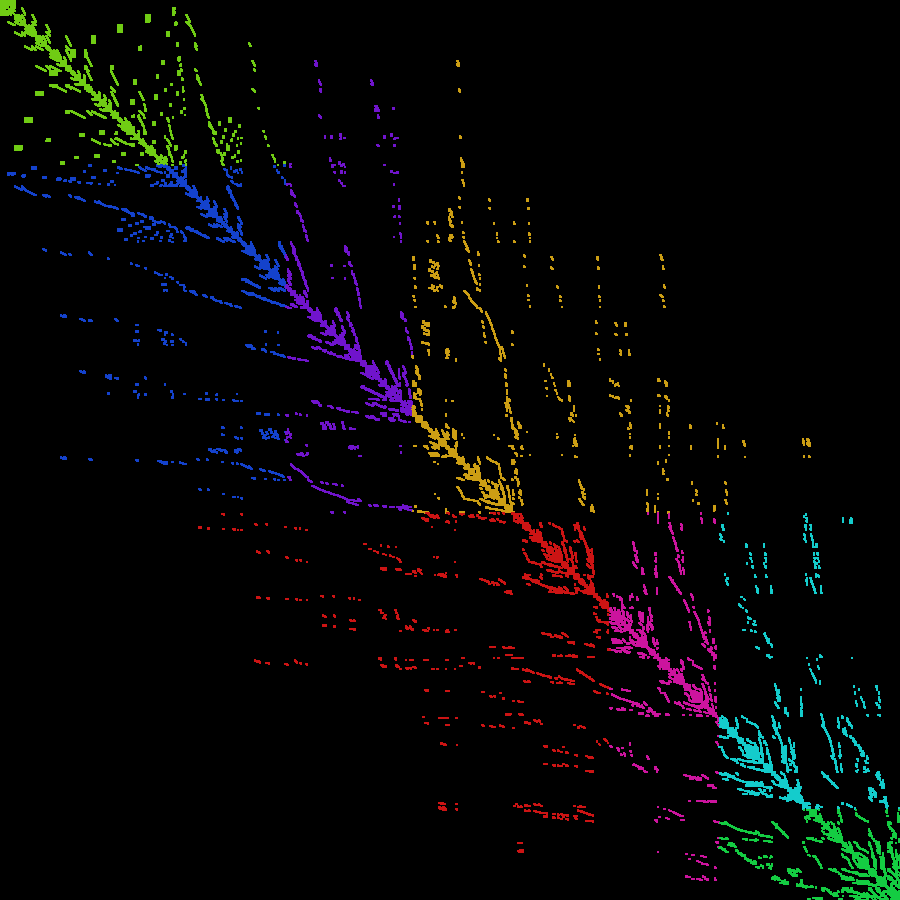
\includegraphics[width=6.5in]{cage12rcb8}
    \caption{Graphical representation of the Cage12 matrix partitioned on an 8-processor system using a two-dimensional partitioning algorithm.  Figure produced by the {\tt IsorropiaVisualizer.py} script provided with the PyTrilinos distribution.}
    \label{fig:cage12rcb8}
  \end{center}
\end{figure}

Another feature of the PyTrilinos Isorropia package is that it installs a script for visualizing partitioned matrices.  Figure~\ref{fig:cage12rcb8} represents output from this script run on the Cage12 matrix~\cite{Cage12} distributed on 8 processors using the Recursive Coordinate Bisection (RCB) algorithm~\cite{RCB}.

\section{Improvements to the Teuchos Module}
\label{sec:teuchos}

As the primary tools package for Trilinos, Teuchos has many useful capabilities.  Some of these capabilities are already provided by standard Python libraries, e.g. command-line option and argument processing, and so are not wrapped in PyTrilinos.  Thus the list of Python interfaces to Teuchos tools is small relative to the package's overall capabilities.  It includes communicators, reference-counted pointers and parameter lists, including XML support.

\subsection{Teuchos Communicators}
\label{sec:teuchos_communicators}

Teuchos communicators are analogous to Epetra communicators: a virtual base class for the purpose of polymorphism, and serial and MPI concrete implementations to enable these two modes of operation.  Unlike an Epetra communicator, Teuchos communicators are templated on an ordinal type and include some advanced programming techniques not allowed under the self-imposed restrictions for Epetra.  There is also a default Teuchos communicator based on an ordinal of type {\tt int}.  PyTrilinos now supports Teuchos communicators.

\subsection{Teuchos Reference-Counted Pointers}
\label{sec:teuchos_rcp}

The new reference-counted pointer support is perhaps the most important improvement to PyTrilinos involving Teuchos (although this improvement is largely invisible to the PyTrilinos user).  The {\tt Teuchos::RCP} class (where RCP stands for reference-counted pointer) is very similar to the {\tt boost::shared\_ptr} class with a few differences (see section 5.14 of~\cite{TeuchosMemMgt}).  These differences include built-in debugging support for {\tt RCP}, the association and retrieval of extra data and other added functionality for {\tt RCP}s, strong and weak references supported by a single {\tt RCP} class versus separate {\tt shared\_ptr} and {\tt weak\_ptr} classes, and slightly lower storage and runtime overhead for {\tt shared\_ptr}s. By developing {\tt RCP}, Trilinos developers avoid a dependency on Boost and more directly control memory management issues.  In the experience of developing PyTrilinos (which has some admittedly complicated use cases), the debugging features of {\tt RCP} have been invaluable.

Reference-counted pointers are a memory management technique that allows objects to be allocated dynamically, to be referenced by other objects, to ensure existence in the presence of such references and to delay deallocation until the last object that holds such a reference has been destroyed.  In pure Python, reference counting is performed automatically without any effort from the programmer whatsoever.  In the Python/C API, the programmer must pay careful attention to reference counting issues, and call incrementing and decrementing macros at the proper times to ensure proper memory management.  In C++, classes such as {\tt boost::shared\_ptr} and {\tt Teuchos::RCP} keep reference counts current automatically via constructors, copy constructors and destructors.

More and more Trilinos packages are adopting the {\tt RCP} as a means of secure memory management.  This has presented a problem for PyTrilinos.  The philosophy of maintaining interfaces with nearly one-to-one mapping between C++ and Python is hard to justify in the face of {\tt RCP}s.  Python programmers would be asked, in what would appear to be a mostly random interface, to sometimes pass an object to a function and other times create a new object, encapsulated in the {\tt RCP} class, in order to pass to a function.  This would be nothing but a source of frustration for Python programmers, who have always been protected from the issue of memory management.

The proper way to implement shared pointers, therefore, is to {\em hide them completely from the Python interface}.  To their credit, SWIG developers have recognized this and have provided an experimental capability to generate interfaces with this property.  But it was not until the release of SWIG version 2.0 that all the bugs were addressed in the Python code generator.

The basic idea is this: if a C++ class defines a type that is at some time accessed as a reference-counted pointer, then all instances of that object within the Python extension module should be stored (internally) as a reference-counted pointer.  The default internal storage method used by SWIG is with a raw pointer that relies upon Python reference counts to determine when the object is deallocated.  By changing the storage technique, this implies that the conversion code for accessing an instance within the generated wrapper code must be specialized in all cases.  In fact, the bulk of the shared pointer support in SWIG is a set of new typemaps that define these new conversions.

In order to provide the desired support for {\tt Teuchos::RCP} that SWIG now provides for {\tt shared\_ptr} classes (in both the {\tt boost} and {\tt std} namespaces), we had to define some macros prior to enabling shared pointer support by applying the {\tt \%include} directive to the SWIG {\tt boost\_shared\_ptr.i} interface file. These macros cause the interface file to refer to {\tt Teuchos::RCP} rather than {\tt shared\_ptr}.  This was far more straightforward than might be expected.  We had to override the output typemaps in order to use the ownership flag that the {\tt RCP} constructor provides, and we had to provide director input and output typemaps, which the SWIG library currently does not implement (see Section~\ref{sec:modelevaluator} for a discussion of SWIG directors).

The end result is that the Python programmer using PyTrilinos will never have to write code that refers to a {\tt Teuchos::RCP}.  Inevitably, a PyTrilinos user will encounter documentation that refers to objects encapsulated by {\tt Teuchos::RCP} (for example, the automatically-generated docstrings include the C++ signatures of the underlying methods).  For this reason, it is very useful for a PyTrilinos user to understand that method arguments or return values that are of type {\tt Teuchos::RCP<object>} in C++, are simply handled as type {\tt object} in Python.  This results in a simplified Python interface relative to the C++ interface with increased readability and no loss of capability.

\subsection{Teuchos Parameter Lists}
\label{sec:teuchos_parameterlists}

At the time of~\cite{PyTrilinos}, {\tt Teuchos::ParameterList}s were supported.  Wherever a {\tt ParameterList} was expected as input, the Python programmer could provide a Python dictionary in its place.  Wherever a {\tt ParameterList} was returned as output, a new type of object, a {\tt PyDictParameterList}, was returned in Python.  This has been simplified and improved somewhat.  Python dictionaries are still accepted as input, but now the {\tt ParameterList} class has been wrapped properly, with the addition of several methods and operators so that it also behaves like a Python dictionary.  This allows access to some {\tt ParameterList} capabilities that Python dictionaries do not possess, such as the usage flags, while still allowing Python programmers to specify {\tt ParameterList}s using highly convenient dictionary syntax.

Another addition to the Teuchos Python module are wrappers for XML classes {\tt XMLObject}, {\tt XMLPa\-rameterListReader}, {\tt XMLParameterListWriter}, {\tt XMLInputSource}, {\tt FileInputSource} and {\tt String\-InputSource}, which together provide full I/O capabilities for {\tt ParameterLists} in XML format.

\section{EpetraExt Model Evaluator}
\label{sec:modelevaluator}

A model evaluator is a concept implemented in both EpetraExt and Thyra that provides a consistent interface for a variety of different models: nonlinear equations, explicit ordinary differential equations (ODEs), implicit ODEs and discrete algebraic equations, unconstrained optimization, equality constrained optimization, general constrained optimization, and function derivatives and sensitivities.  Often, scientists will want to evaluate a model in more than one of these supported modes, and so a single interface becomes extremely useful.  Several Trilinos solver packages now accept model evaluators, so this approach provides a high degree of functionality.  The {\tt ModelEvaluator} class in EpetraExt is now supported in PyTrilinos.

The {\tt ModelEvaluator} class is a virtual base class with a pure virtual {\tt modelEval()} method that must be implemented by a derived class.  A solver or optimization object that has a ModelEvaluator interface will call this {\tt modelEval()} method whenever a model evaluation is required.

SWIG supports the use case of writing such a derived class in Python, including the {\tt modelEval()} method.  This is known as cross-language polymorphism and works as follows:  SWIG generates a C++ class that inherits from the {\tt ModelEvaluator} class that provides compilable code for all virtual methods.  Such a class is known as a director class and such methods are known as director methods.  This is because the class is wrapped with a Python interface and that interface is checked dynamically for implementations of the director methods (such as {\tt modelEval()}).  If such Python methods are found, the underlying C++ methods direct execution to the Python code.  If not, the default C++ implementation will be called, or for a pure virtual method, an exception raised.

The Python interface for the EpetraExt {\tt ModelEvaluator} class was a challenge to develop because the {\tt ModelEvaluator} makes heavy use of nested classes.  This is the one case of C++ code that is not supported by SWIG.  There are workarounds for this situation suggested by SWIG developers, but the {\tt ModelEvaluator} class is complex enough that it resisted these workarounds.  The ultimate solution was to redefine the nested classes as non-nested pure Python classes and then write typemaps that convert these Python arguments to the appropriate underlying C++ types.

{\tt ModelEvaluator} classes are useful only if there are corresponding solver objects which support the ModelEvaluator interface.  To date only the NOX nonlinear solver package supports the ModelEvaluator interface within PyTrilinos.

\section{Vision for Second-Generation Packages}
\label{sec:vision}

First-generation Trilinos packages are designed around the Epetra package, which provides distributed linear algebra classes such as vectors, multivectors, operators, and sparse matrices.  Development of Epetra began over a decade ago, when variations in C++ compilers from platform to platform were considerable.  For this reason, Epetra was designed without templates or namespaces, to maximize portability.  As a result, Epetra scalar data is always {\tt double} and ordinals are always {\tt int}.  In the intervening decade, needs have inevitably arisen for complex and single precision scalar data (especially for GPUs) and {\tt long} ordinal data (as platforms and global problem sizes have grown).  To address these needs, a second-generation linear algebra services package, Tpetra (Templated Petra) has been developed, with template arguments for scalar data, local ordinals and global ordinals.

PyTrilinos provides wrappers to a significant subset of first-generation packages.  This includes Teuchos, which has evolved to support both first and second-generation packages, and Anasazi, which was designed from its origins to both utilize templates and interface to Epetra.  But Tpetra does not yet have a PyTrilinos interface, and so most of the second-generation packages do not either.

C++ templates present a challenge to designing Python interfaces that wrap such code.  This stems from the fact that C++ implements templates with a heavy dependence on syntax while the same concept is implemented dynamically in Python without syntax.  In other words, because Python function and method arguments do not specify types, any argument type will work as long there is support for all of the operators and functions applied to that argument.  Thus Python ``templates'' are implicit and implemented at run time, while C++ templates are explicit and implemented at compile time.  As a Python interface to compiled code, Python extensions must link to a finite set of concrete instantiations of C++ template code, which makes this use case far less generic than pure Python is.

The SWIG method for generating wrapper code for templates is to parse template code internally but only produce wrappers for concrete instantiations, each one requiring a unique name.  As a simple example of this, consider an attempt to wrap the C++ {\tt Tpetra::Vector} class.  We will focus on a subset of a significant simplification of the class that will expose wrapping issues of concern:
\begin{verbatim}
    namespace Tpetra {
        template< class T >
        class Vector {
            Vector(size_type n = 0);
        };
    }
\end{verbatim}
We can instantiate {\tt Tpetra::Vector} with any type T, and this will produce an array of data of type T.  We would like a Python interface that gives us access to this class with a variety of types supported.  To wrap this class with SWIG, one might include the following in the SWIG interface file:
\begin{verbatim}
    %template(Vector_int   ) Tpetra::Vector<int>;
    %template(Vector_long  ) Tpetra::Vector<long>;
    %template(Vector_float ) Tpetra::Vector<float>;
    %template(Vector_double) Tpetra::Vector<double>;
\end{verbatim}
This would produce a Python extension module with definitions for four independent classes:
\begin{verbatim}
    from PyTrilinos import Tpetra
    n = 10
    vi = Tpetra.Vector_int(n)
    vl = Tpetra.Vector_long(n)
    vf = Tpetra.Vector_float(n)
    vd = Tpetra.Vector_double(n)
\end{verbatim}
This interface is decidedly not ``Pythonic.''  It is also not scalable; C++ code that utilizes multiple template parameters would quickly result in names that are too long or too cryptic to be usable or readable.

A preferable interface would consist of a single Python class named Vector.  This would require the addition of a technique to specify the scalar data type.  The NumPy module has already addressed this issue with the utilization of {\tt dtype} arguments, and so a similar solution would be both familiar to scientific Python programmers and compatible with NumPy:
\begin{verbatim}
    from PyTrilinos import Tpetra
    n = 10
    vi = Tpetra.Vector(n, dtype="i")
    vl = Tpetra.Vector(n, dtype="l")
    vf = Tpetra.Vector(n, dtype="f")
    vd = Tpetra.Vector(n, dtype="d")
\end{verbatim}
To accomplish this in SWIG would require the development of a complete new class in C++ that is not itself templated, but is capable of internally storing several templated Vector classes of different (predefined) types, only one of which would be active with allocated data.  With this paradigm, SWIG loses some of its advantages.  We are no longer targeting a nearly one-to-one interface between C++ and Python and must spend considerable effort designing a new interface.  This interface definition makes other wrapping tools, such as SIDL/Babel, Boost.Python or Cython much more attractive.  Cython in particular might be particularly adept at helping to develop ``Pythonic'' interfaces.

At the time of final submission of this paper, Enthought, Inc. has been awarded a Department of Energy (DOE) Small Business Innovation Research (SBIR) Phase I grant researching and developing this very issue in consultation with Sandia.  Cython will be used to develop the Python interface to {\tt Tpetra::Vector} and other elements of the Tpetra package.  This raises the question of whether interfaces developed with SWIG can be compatible with interfaces developed with Cython.  If so, Cython will be an attractive approach for wrapping second-generation Trilinos packages.  If not, the sheer inertia of SWIG-wrapped PyTrilinos packages may dictate continuing to use SWIG to generate the Python interfaces.  The SBIR research should answer this and related questions.

\section{Concluding Remarks}
\label{sec:concluding remarks}

The Trilinos Project is now over a decade old and has seen massive growth in that time.  Beginning with three packages for linear algebra services, iterative solvers and preconditioners, Trilinos has grown to now encompass 50 packages in its current release, with more planned for the future.  It has grown from a suite of solver technologies to a suite of simulation tools, now including meshing, discretizations, partitioning, load balancing, automatic differentiation, optimization and much more.  As C++ compilers have matured, more advanced programming techniques have been employed.  As lessons have been learned regarding object-oriented design for scientific computing, those lessons have been deployed in the code base.

These advances, coupled with the need for stable interfaces, have inevitably led to the development of second-generation packages such as Tpetra, Belos and Ifpack2.  PyTrilinos provides Python interfaces to first-generation packages, with an emphasis on Epetra and those packages that process Epetra objects.  As the second-generation packages mature, we expect pressure to mount to provide Python interfaces to them.  Tpetra vectors, with their support of multiple data types, are more powerful than Epetra vectors, with their restriction to double precision.  This makes Tpetra vectors more like NumPy arrays, with the added capability of distribution over parallel computing architectures.  Thus Tpetra and the packages that use it are obvious candidates for Python wrappers.  So while PyTrilinos currently provides an impressive set of capabilities, it is also at a crossroads, facing a large new set of potential capabilities to provide in the form of second-generation Trilinos packages.  The good news is that initial funding has been obtained to enable this upgrade.

\bibliographystyle{plain}
\bibliography{PyTrilinos}

\end{document}
\end
